\documentclass{ximera}
%% handout
%% nohints
%% space
%% newpage
%% numbers

%% You can put user macros here
%% However, you cannot make new environments

\graphicspath{{./}{firstExample/}{secondExample/}}

\usepackage{url}
\usepackage{tikz}
\usepackage{tkz-euclide}
\usetkzobj{all}


\tikzstyle geometryDiagrams=[ultra thick,color=blue!50!black]
\pgfplotsset{compat=1.8}
  \usepackage[T1]{fontenc}
  \usepackage[utf8x]{inputenc} %% we can turn off input when making a master document

\prerequisites{none}


\title{Inflation}

\begin{document}
\begin{abstract}
We examine the concept of inflation.
\end{abstract}
\maketitle

\begin{quote}
It is a way to take people's wealth from them without having to openly raise taxes. Inflation is the most universal tax of all. --- Thomas Sowell
\end{quote}

Inflation is a rise in the prices of goods and services over time. This has the effect of devaluing currency so that $\$1.00$ in the future is worth less, or has less buying power, than $\$1.00$ now. There are several different mechanisms that appear to influence inflation as well as a variety of controls that governments and central banks use to try to control it. When one industry raises prices, because of increased demand, reduced supply, or simply to increase profits, the effect is that others must now pay more for the goods and services provided by that industry than before. Spending more may require buyers to borrow more than before, or to work more, or to engage in other activities that increase the amount of money in circulation. The end result is higher prices and more money in circulation (the latter possibly leading to higher wages down the road).\footnote{A brief explanation of some causes of inflation written for the public is available \href{http://www.forbes.com/sites/johntharvey/2011/05/30/what-actually-causes-inflation/}{here}.}

One stark example of inflation occurred in the Weimar Republic (modern-day Germany) in the years between World War $1$ and World War $2$. At the conclusion of World War $1$, Germany was required to pay large amounts of money to the victorious countries as \emph{reparations}. The victors required these payments be made in hard currency, such as gold. On top of this, Germany had financed a large part of the war by either borrowing money or simply printing more of its own money (Marks). As a result of these factors, the Weimar government was forced to print more currency to purchase gold or trade for foreign currency to pay the reparations. There was also a great deal of political turmoil in Weimar. Potential trading partners became wary of the instability and began charging more and more Marks for the same goods (such as gold), requiring the Weimar government to print even more money. A vicious spiral of decreasing currency value and increasing currency volume eventually ensued, set against the backdrop of political assassinations, distrust of the government, class warfare, and rising anti-Semitism. The inflation was so bad that some businesses began paying workers in newly invented local currencies while those who were still paid in Marks spent their pay immediately to avoid the inevitable depreciation in its worth. Eventually, the government was unable to make its reparation payments in hard currency and in retaliation France occupied Weimar's industrial center, which led to a strike by the workers. Crisis after crisis\footnote{\href{http://www.businessinsider.com/weimar-the-real-story-of-the-devastating-collapse-that-haunts-the-eurozone-today-2012-10?op=1}{Weimar's Hyperinflation}} led to more and more inflation, increasing poverty, further instability, and set the stage for the ascension of Adolf Hitler in the $1930$'s.

As an illustration of how severe the inflation was, the following table shows approximately how many Marks were required to purchase $1$ gram of gold during the hyperinflation.\footnote{\href{http://en.wikipedia.org/wiki/Hyperinflation}{http://en.wikipedia.org/wiki/Hyperinflation}}

\begin{image}
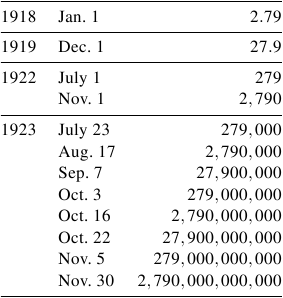
\includegraphics{InflationTable1.png}
%\begin{tabular}{@{}llr@{}}\toprule
%\textbf{$1918$} & Jan.\ $1$ & $2.79$ \\\midrule
%\textbf{$1919$} & Dec.\ $1$ & $27.9$\\\midrule
%\textbf{$1922$} & July $1$ & $279$\\
% & Nov.\ $1$ & $2,790$\\\midrule
% \textbf{$1923$} & July $23$ & $279,000$\\
% & Aug.\ $17$ & $2,790,000$\\
% &  Sep.\ $7$ & $27,900,000$\\
% & Oct.\ $3$ & $279,000,000$\\
% & Oct.\ $16$ & $2,790,000,000$\\
% &  Oct.\ $22$ & $27,900,000,000$\\
% & Nov.\ $5$ & $279,000,000,000$\\
% & Nov.\ $30$ & $2,790,000,000,000$\\\bottomrule
%\end{tabular}
\end{image}

\begin{question}
If it cost a family of $4$ in the Weimar Republic $60$ Marks for a week's worth of food on Dec.\ $1$, $1919$, about how much would the same amount of food cost them on Nov.\ $5$, $1923$?

\begin{multipleChoice}
\choice{$600,000$ Marks}
\choice{$6$ million Marks}
\choice{$600$ million Marks}
\choice{$6$ billion Marks}
\choice[correct]{$600$ billion Marks}
\end{multipleChoice}

\begin{hint}
It might be useful to use a proportion, such as \[ \frac{\text{Old price of food}}{\text{Old price of gold}} = \frac{\text{New price of food}}{\text{New price of gold}}\]
\end{hint}
\end{question}

Other countries have experienced hyperinflation since the debacle in Weimar. At the close of World War $2$, Hungary experienced inflation so bad that prices doubled every $15$ hours $36$ minutes. More recently, Zimbabwe experienced a doubling of prices every $24$ hours and $42$ minutes during $2008$.\footnote{\href{http://www.cato.org/zimbabwe}{Zimbabwe's Hyperinflation}} Usually, hyperinflation is only stopped when the existing currency is declared worthless and replaced with a new currency, sometimes adopted from a large, stable economy elsewhere in the world.

In the U.S., the Bureau of Labor Statistics publishes a monthly statistic called the Consumer Price Index (CPI).\footnote{There are actually several statistics under the umbrella-term Consumer Price Index, narrowed by region or subgroup of the population. The most general,and the one we will refer to as the CPI, is the All Items Consumer Price Index for All Urban Consumers for the U.S.\ City Average. \href{http://www.bls.gov/cpi/cpifaq.htm}{http://www.bls.gov/cpi/cpifaq.htm}} The CPI is an attempt to measure the relative change in costs a consumer would experience over time, based on a specific reference point. The CPI uses the years $1982-1984$ as a base from which to calculate the change in prices. The index is set to $100$ for those years and so values in subsequent years can tell us the percentage increase in costs since that time. For example, the CPI in May $2014$ was $237.9$, meaning that prices had \emph{increased} approximately $137.9\%$ since $1982-1984$.

\begin{question}
What would a family's annual income need to be in May $2014$ to sustain the same standard of living as $\$25,000$ did in $1983$?

$\$$\answer{$59475$}

\begin{hint}
The amount of \emph{increase} is $137.9\%$ of $\$25,000$, but the total is the amount of increase plus the original amount.
\end{hint}
\end{question}

\begin{question}
In December of $2003$, the CPI was $184.3$. A decade later, in December of $2013$, the CPI was $233.049$. According to these values, by what percent had prices increased during that ten year span?


\begin{multipleChoice}
\choice{$48.7\%$}
\choice[correct]{$26.5\%$}
\choice{$20.9\%$}
\choice{$79.1\%$}
\choice{$1.26\%$}
\end{multipleChoice}

\begin{hint}
The CPI values for $2003$ and $2013$ are comparisons to $1982-1984$. You want a comparison of $2013$ to $2003$.
\end{hint}

\begin{hint}
You can use the equation from the section on percentages, \[ \text{Percentage}=\frac{\text{Part}}{\text{Whole}}\times 100 \]
\end{hint}

\end{question}
\end{document}
